\documentclass{beamer}
\usepackage[utf8]{inputenc}

\usetheme{Madrid}
\usecolortheme{default}
\usepackage{amsmath,amssymb,amsfonts,amsthm}
\usepackage{txfonts}
\usepackage{tkz-euclide}
\usepackage{listings}
\usepackage{adjustbox}
\usepackage{array}
\usepackage{tabularx}
\usepackage{gvv}
\usepackage{lmodern}
\usepackage{circuitikz}
\usepackage{tikz}
\usepackage{graphicx}
\usepackage{mathtools}
\setbeamertemplate{page number in head/foot}[totalframenumber]

\usepackage{tcolorbox}
\tcbuselibrary{minted,breakable,xparse,skins}



\definecolor{bg}{gray}{0.95}
\DeclareTCBListing{mintedbox}{O{}m!O{}}{%
  breakable=true,
  listing engine=minted,
  listing only,
  minted language=#2,
  minted style=default,
  minted options={%
    linenos,
    gobble=0,
    breaklines=true,
    breakafter=,,
    fontsize=\small,
    numbersep=8pt,
    #1},
  boxsep=0pt,
  left skip=0pt,
  right skip=0pt,
  left=25pt,
  right=0pt,
  top=3pt,
  bottom=3pt,
  arc=5pt,
  leftrule=0pt,
  rightrule=0pt,
  bottomrule=2pt,
  toprule=2pt,
  colback=bg,
  colframe=orange!70,
  enhanced,
  overlay={%
    \begin{tcbclipinterior}
    \fill[orange!20!white] (frame.south west) rectangle ([xshift=20pt]frame.north west);
    \end{tcbclipinterior}},
  #3,
}
\lstset{
    language=C,
    basicstyle=\ttfamily\small,
    keywordstyle=\color{blue},
    stringstyle=\color{orange},
    commentstyle=\color{green!60!black},
    numbers=left,
    numberstyle=\tiny\color{gray},
    breaklines=true,
    showstringspaces=false,
}


\title 
{4.8.6}
\date{September 29, 2025}


\author 
{Dhanush Kumar A - AI25BTECH11010}



\begin{document}
\frame{\titlepage}
\begin{frame}{Question}

Find the coordinates of the foot of the perpendicular $\vec{Q}$ drawn from $P(3,2,1)$ to the
plane $2x - y + z + 1 = 0$. Also find the distance $\vec{P}\vec{Q}$ and the image of the point $\vec{P}$
treating this plane as a mirror.
\end{frame}
\begin{frame}{Solution}

The point and the plane normal are
\begin{align}
\vec{P} &= \myvec{3\\2\\1}, & \vec{n} &= \myvec{2\\-1\\1},
\end{align}

\begin{align}
\vec{n}^T\vec{x} = -1.
\end{align}

Let $\vec{Q}$ be the foot of the perpendicular from $\vec{P}$ to the plane and let $\lambda$ be the scalar such that
\begin{align}
\vec{P}-\vec{Q} &= \lambda\vec{n}\\
\vec{n}^T\vec{Q} &= -1. 
\end{align}
 we have $\vec{Q}=\vec{P}-\lambda\vec{n}$.
 Therefore,
\begin{align}
\vec{n}^T(\vec{P}-\lambda\vec{n}) &= -1 \\
\vec{n}^T\vec{P} - \lambda\|\vec{n}\|^2 &= -1.
\end{align}
\end{frame}
\begin{frame}{Solution}

Thus
\begin{align}
5 - 6\lambda &= -1 \quad\Rightarrow\quad \lambda = -1.
\end{align}
Therefore
\begin{align}
\vec{Q} &= \vec{P}-\lambda\vec{n} = \myvec{3\\2\\1} - (-1)\myvec{2\\-1\\1}
= \myvec{1\\3\\0}.
\end{align}

Distance:
\begin{align}
PQ = \|\vec{P}-\vec{Q}\| = \|\lambda\vec{n}\| = |\lambda|\|\vec{n}\| = 1\cdot\sqrt{6}=\sqrt{6}.
\end{align}

Image of $\vec{P}$ in the plane (reflection) is
\begin{align}
\vec{R} &= 2\vec{Q} - \vec{P} = 2\myvec{1\\3\\0} - \myvec{3\\2\\1} = \myvec{-1\\4\\-1}.
\end{align}

\bigskip
\noindent\textbf{Answer:} \(
\vec{Q}=(1,3,0),\; PQ=\sqrt{6},\; \vec{R}=(-1,4,-1).
\)
\end{frame}
\begin{frame}{Plot}
    \centering
    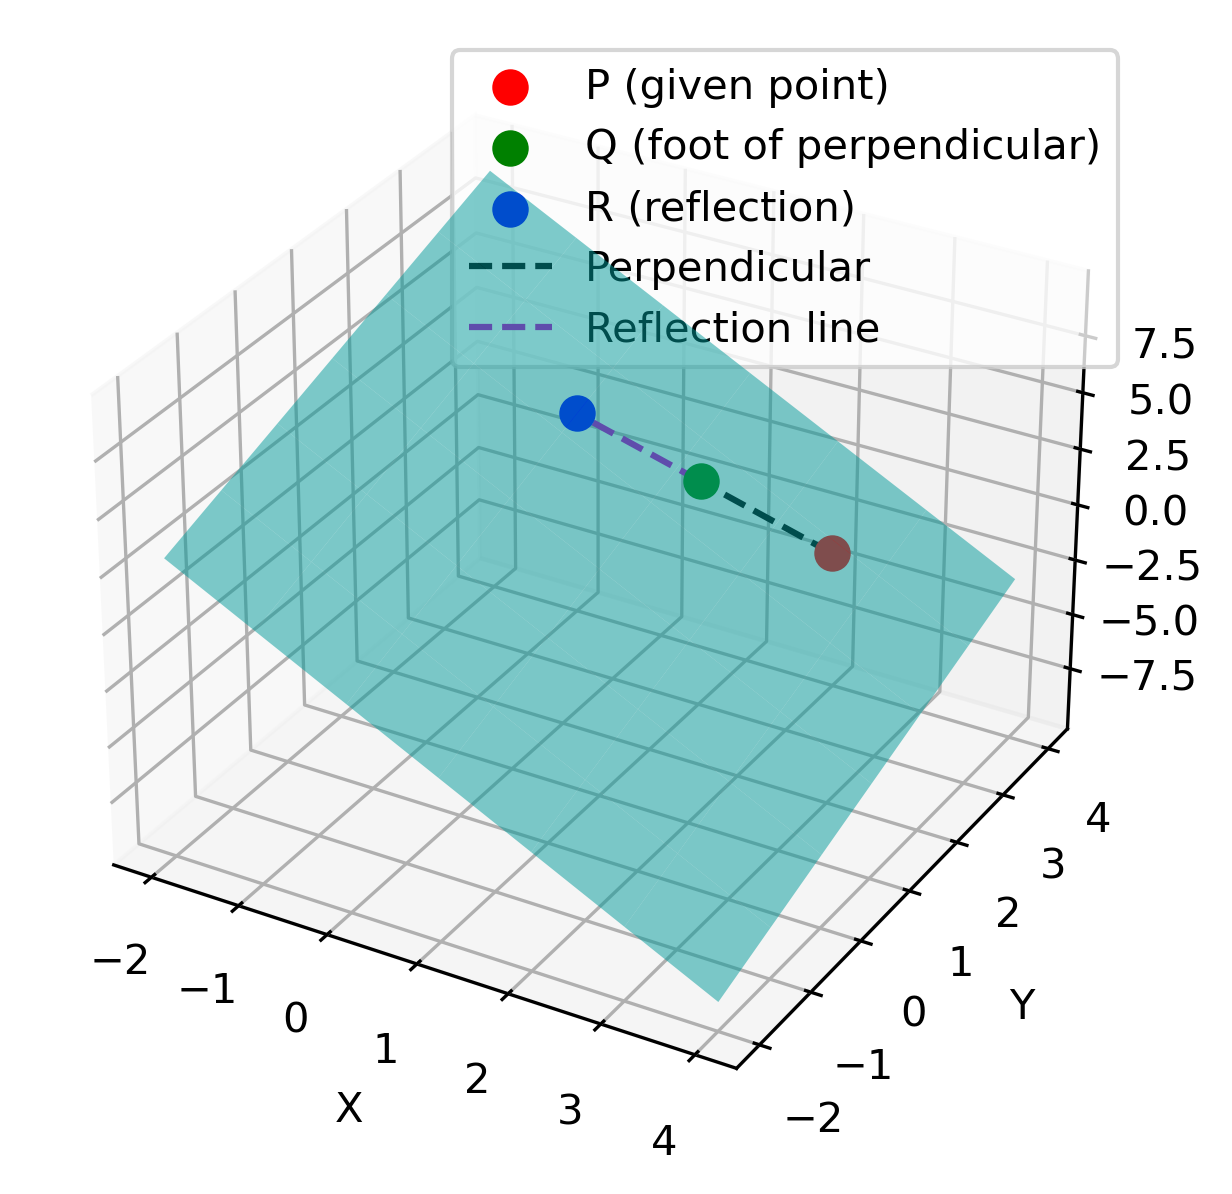
\includegraphics[width=\columnwidth, height=0.8\textheight, keepaspectratio]{../figs/point_plane.png}     
\end{frame}


\begin{frame}[fragile]                            
\frametitle{Python code - To find n }                
\begin{lstlisting}



import numpy as np
import matplotlib.pyplot as plt
import os
from mpl_toolkits.mplot3d import Axes3D

# Function to compute foot of perpendicular, distance, and reflection
def solve_point_plane(P, n, d):
    P = np.array(P, dtype=float)
    n = np.array(n, dtype=float)

    # λ = (n^T P - d) / (n^T n)
    lam = (np.dot(n, P) - d) / np.dot(n, n)

    # Foot of perpendicular
    Q = P - lam * n
\end{lstlisting}
\end{frame}


\begin{frame}[fragile]                            
\frametitle{Python code - To find n }                
\begin{lstlisting}


    # Distance
    dist = abs(lam) * np.linalg.norm(n)

    # Reflection
    R = 2 * Q - P

    return lam, Q, dist, R


# ---------------- MAIN CODE ----------------
P = np.array([3, 2, 1])
n = np.array([2, -1, 1])
d = -1   # Plane equation: n^T x = -1

# Solve
lam, Q, dist, R = solve_point_plane(P, n, d)
\end{lstlisting}
\end{frame}


\begin{frame}[fragile]                            
\frametitle{Python code - To find n }                
\begin{lstlisting}

print("λ =", lam)
print("Foot of perpendicular Q =", Q)
print("Distance =", dist)
print("Reflection R =", R)
\end{lstlisting}
\end{frame}

\begin{frame}[fragile]                            
\frametitle{Python code - Plotting the Plane}                
\begin{lstlisting}
# ---------- Plotting ----------
fig = plt.figure()
ax = fig.add_subplot(111, projection='3d')

# Create a grid for the plane
xx, yy = np.meshgrid(range(-2, 5), range(-2, 5))
zz = (-d - n[0]*xx - n[1]*yy) / n[2]

# Plot the plane surface
ax.plot_surface(xx, yy, zz, alpha=0.5, color='cyan')

# Plot points P, Q, R
ax.scatter(*P, color='red', s=60, label='P (given point)')
ax.scatter(*Q, color='green', s=60, label='Q (foot of perpendicular)')
ax.scatter(*R, color='blue', s=60, label='R (reflection)')
\end{lstlisting}
\end{frame}

\begin{frame}[fragile]                            
\frametitle{Python code - Plotting the Plane}                
\begin{lstlisting}

# Draw perpendicular line P-Q
ax.plot([P[0], Q[0]], [P[1], Q[1]], [P[2], Q[2]], 'k--', label='Perpendicular')

# Draw line Q-R
ax.plot([Q[0], R[0]], [Q[1], R[1]], [Q[2], R[2]], 'm--', label='Reflection line')

# Labels
ax.set_xlabel("X")
ax.set_ylabel("Y")
ax.set_zlabel("Z")
ax.legend()

# ---------- Save figure ----------
os.makedirs("figs", exist_ok=True)   # create folder if not exists
save_path = os.path.join("../figs", "point_plane.png")
plt.savefig(save_path, dpi=300, bbox_inches='tight')


plt.close(fig)  # Close figure instead of showing
\end{lstlisting}

\end{frame}
\begin{frame}{Plot-Using  Python}
    \centering
    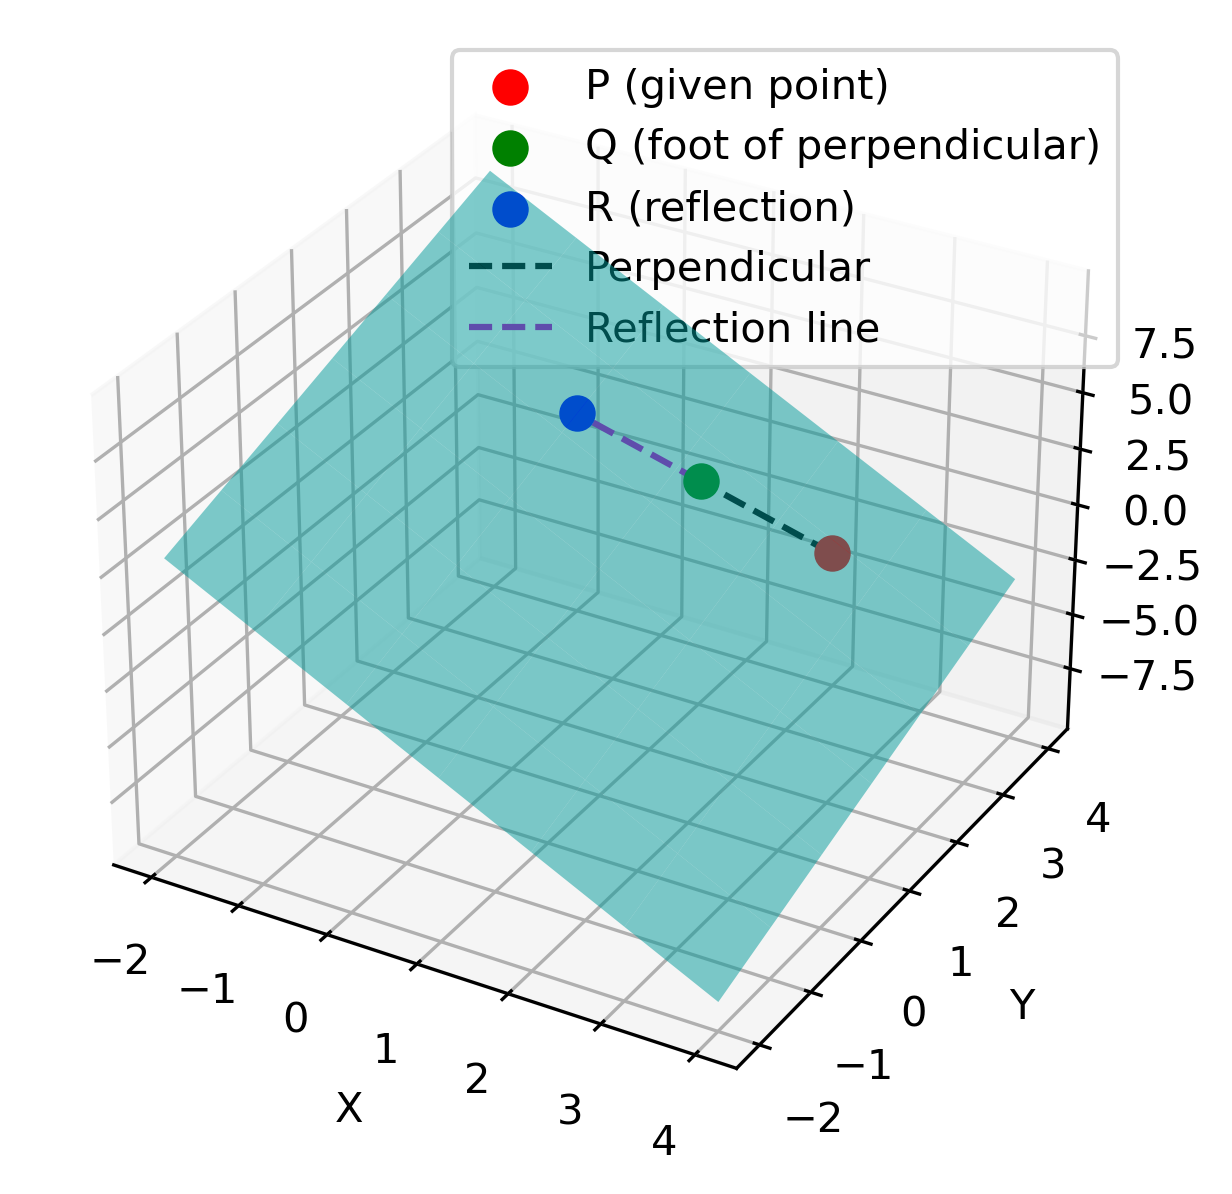
\includegraphics[width=\columnwidth, height=0.8\textheight, keepaspectratio]{../figs/point_plane.png}     

\end{frame}

\begin{frame}[fragile]                            
\frametitle{C code - Solving}                
\begin{lstlisting}

#include <stdio.h>
#include <stdlib.h>
#include <math.h>
#include "/home/dhanush-kumar-a/ee1030-2025/ai25btech11010/matgeo/4.8.6/codes/libs/matfun.h"

// Function to compute distance and reflection
// Inputs: P (3x1), n (3x1), d
// Outputs: distance (pointer), R (3x1 array)
void point_plane_info(double **P, double **n, double d, double *distance, double *R) {
    // Compute lambda
    double lam = (Matdot(n,P,3) - d)/(Matdot(n,n,3));

    // Compute foot of perpendicular Q = P - lambda*n
    double **Q = Matsub(P, Matscale(n,3,1,lam), 3,1);
\end{lstlisting}
\end{frame}

\begin{frame}[fragile]                            
\frametitle{C code - Solving}                
\begin{lstlisting}

    // Compute distance = |lambda| * ||n||
    *distance = fabs(lam) * Matnorm(n,3);

    // Compute reflection R = 2*Q - P
    double **Rmat = Matsub(Matscale(Q,3,1,2.0), P, 3,1);

    // Copy results to output array
    for(int i=0;i<3;i++)
        R[i] = Rmat[i][0];

    // Free memory
    for(int i=0;i<3;i++){
        free(Q[i]);
        free(Rmat[i]);
    }
    free(Q);
    free(Rmat);
}


\end{lstlisting}
\end{frame}

	
\begin{frame}[fragile]                              
	\frametitle{Python code -Ploting the plane using c function} 
	\begin{lstlisting}

import ctypes
import numpy as np
import matplotlib.pyplot as plt
import os


# Load the shared library (use absolute path if needed)
lib = ctypes.CDLL("./main.so")  # or absolute path

# Prepare point P and normal n
P_vals = [3.0, 2.0, 1.0]
n_vals = [2.0, -1.0, 1.0]

# Allocate pointers for P and n (double**)
P = (ctypes.POINTER(ctypes.c_double) * 3)()
n = (ctypes.POINTER(ctypes.c_double) * 3)()
for i in range(3):
    P[i] = ctypes.pointer(ctypes.c_double(P_vals[i]))
    n[i] = ctypes.pointer(ctypes.c_double(n_vals[i]))
\end{lstlisting}
\end{frame}

\begin{frame}[fragile]                            
\frametitle{Python code - Plotting the Plane}                
\begin{lstlisting}

# Prepare outputs
distance = ctypes.c_double()
R = (ctypes.c_double * 3)()

# Call the C function
lib.point_plane_info(
    P,                 # double**
    n,                 # double**
    ctypes.c_double(-1.0),  # plane constant d
    ctypes.byref(distance),  # double* output
    R                  # double* output
)

# Convert R to numpy array
R_vals = np.array([R[i] for i in range(3)])
P_arr = np.array(P_vals)
n_arr = np.array(n_vals)
d = -1.0
\end{lstlisting}
\end{frame}

\begin{frame}[fragile]                            
\frametitle{Python code - Plotting the Plane}                
\begin{lstlisting}

# Compute Q = foot of perpendicular
lam = (np.dot(n_arr, P_arr) - d) / np.dot(n_arr, n_arr)
Q_arr = P_arr - lam * n_arr

# Print results
print("Distance from P to plane:", distance.value)
print("Foot of perpendicular Q:", Q_arr)
print("Reflection R:", R_vals)

# --- Plotting ---
fig = plt.figure()
ax = fig.add_subplot(111, projection='3d')
\end{lstlisting}
\end{frame}

\begin{frame}[fragile]                            
\frametitle{Python code - Plotting the Plane}                
\begin{lstlisting}

# Plot points P, Q, R
ax.scatter(*P_arr, color='blue', label='P')
ax.scatter(*Q_arr, color='green', label='Q (foot)')
ax.scatter(*R_vals, color='red', label='R (reflection)')

# Plot plane
xx, yy = np.meshgrid(np.linspace(0,5,10), np.linspace(0,5,10))
zz = (-n_arr[0]*xx - n_arr[1]*yy + d)/n_arr[2]
ax.plot_surface(xx, yy, zz, alpha=0.3, color='orange')

ax.set_xlabel('X')
ax.set_ylabel('Y')
ax.set_zlabel('Z')
ax.legend()
ax.set_title("Point, Foot of Perpendicular, Reflection, Plane")

# Save figure
plt.savefig("../figs/point_plane_plot.png", dpi=300)
plt.show()
\end{lstlisting}                               
\end{frame}

\begin{frame}{Plot-Using  Python and C}
    \centering
    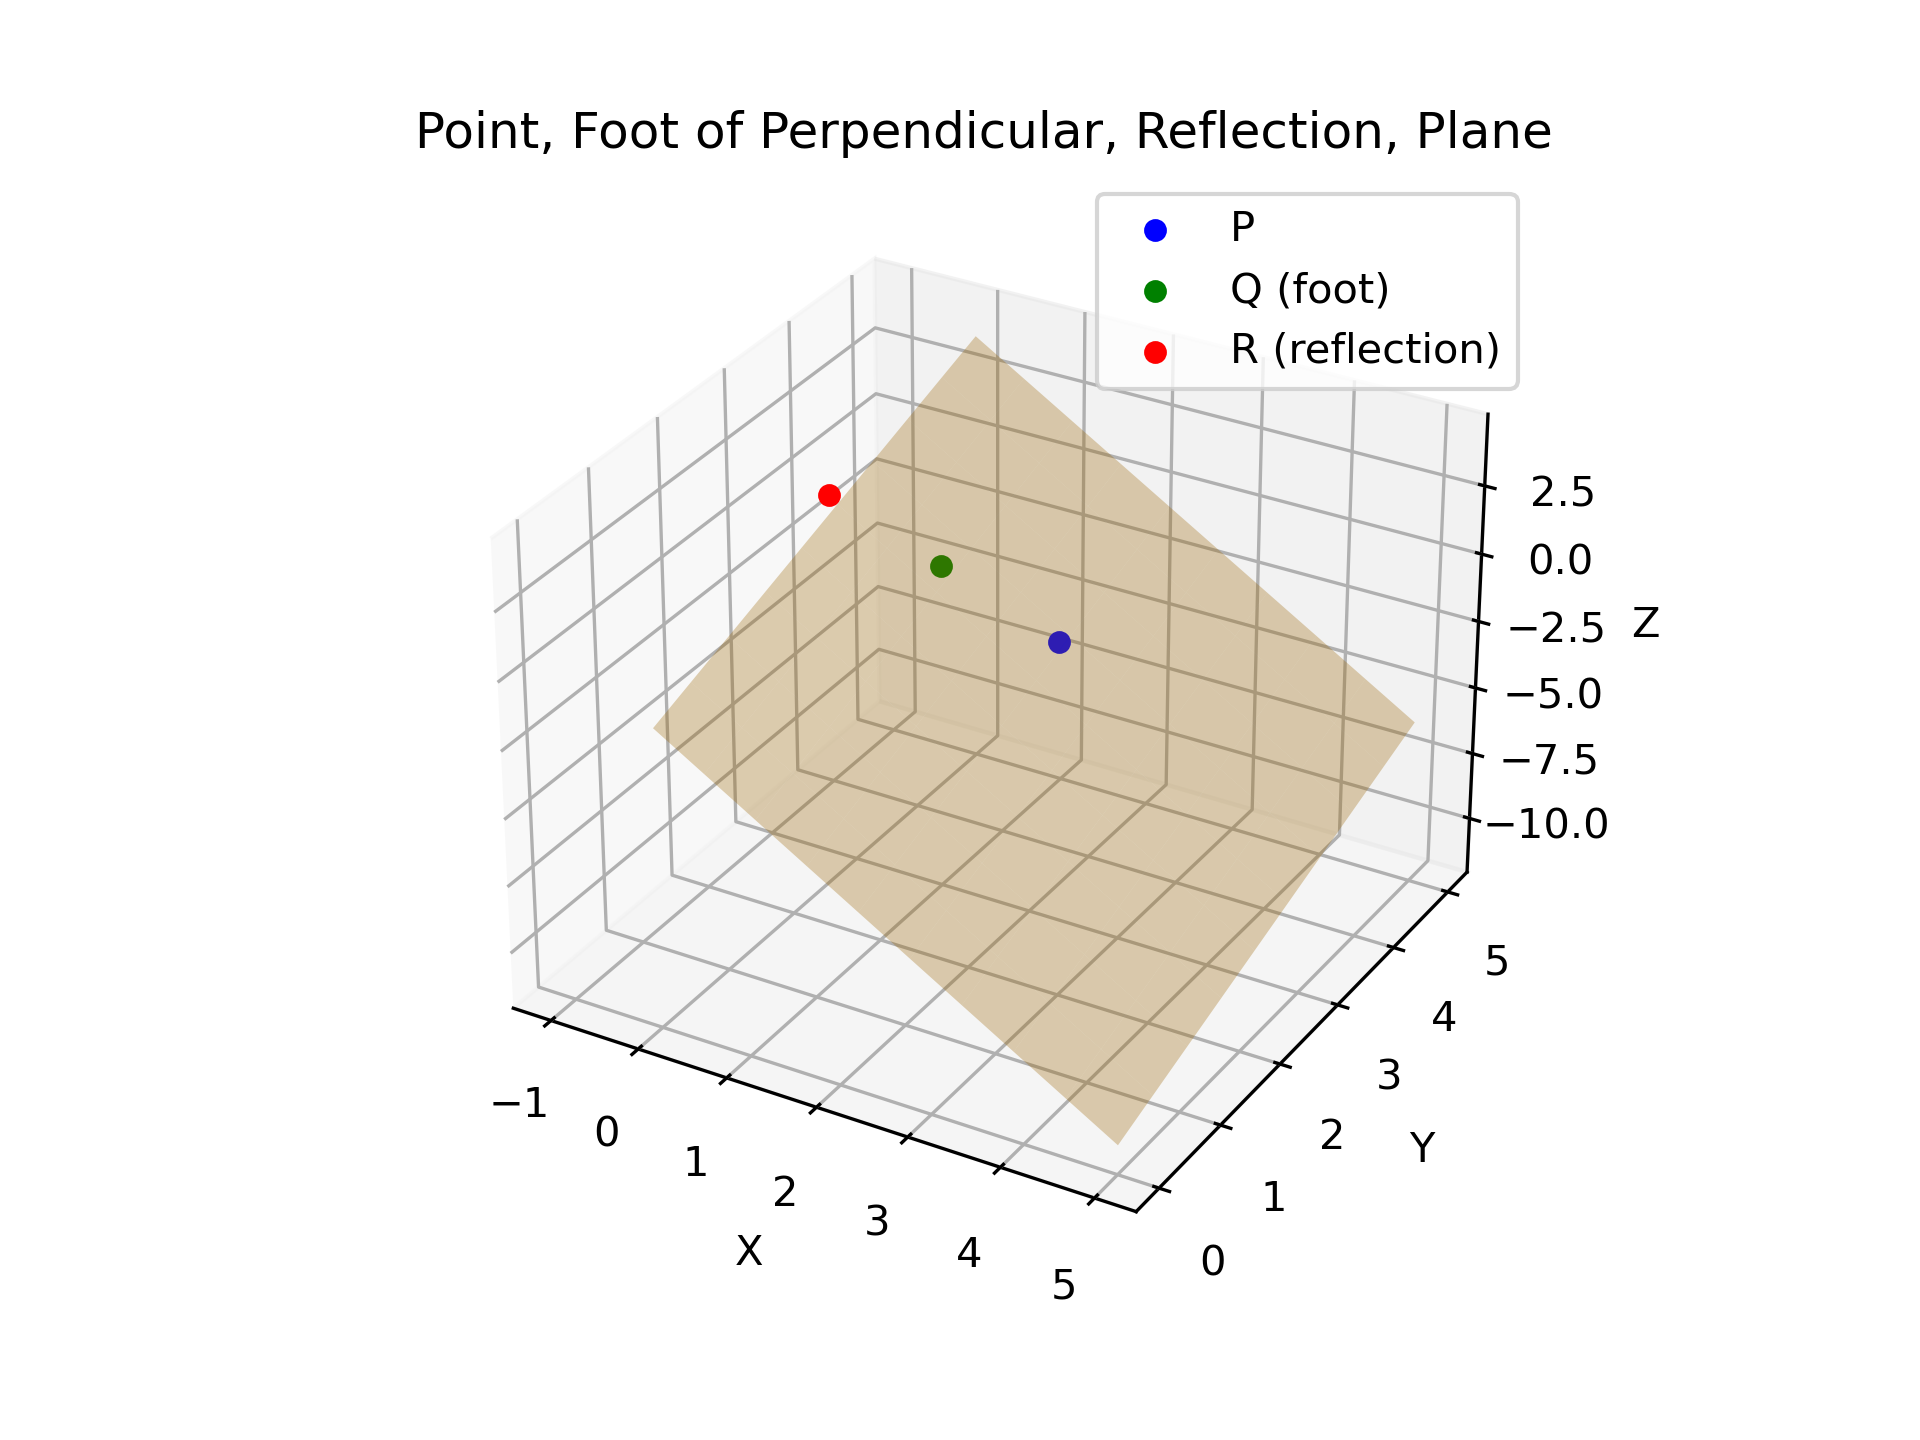
\includegraphics[width=\columnwidth, height=0.8\textheight, keepaspectratio]{../figs/point_plane_plot.png}     
\end{frame}

	


\end{document}

